\chapter{Results}
\label{chap:chap-four}
\section{Node ability test}
\subsection{Nodes upload test}
 Test 40,000 nodes'(random select) speed  three times a day (3A.M. Figure \ref{fig_20} ,
12A.M. Figure \ref{fig_21} , 9 P.M. Figure \ref{fig_22})
by uploading a big file (1GB) to the server, using TCP connect.


\begin{figure}[htbp]
\centering
	  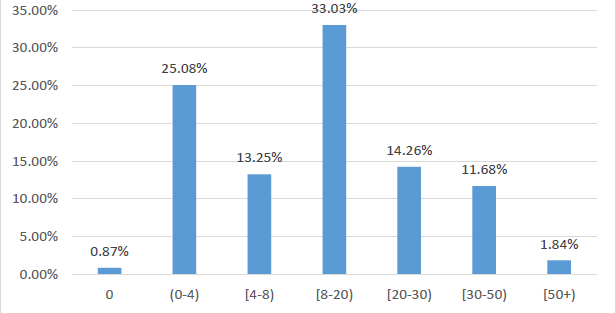
\includegraphics[width=\textwidth]{fig_20.png}
    \caption{3 A.M.}
 \label{fig_20}
\end{figure}

\begin{figure}[htbp]
\centering
	  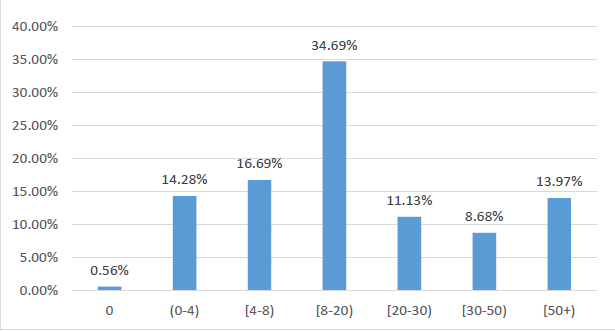
\includegraphics[width=\textwidth]{fig_21.png}
    \caption{12 A.M.}
 \label{fig_21}
\end{figure}

\begin{figure}[htbp]
\centering
	  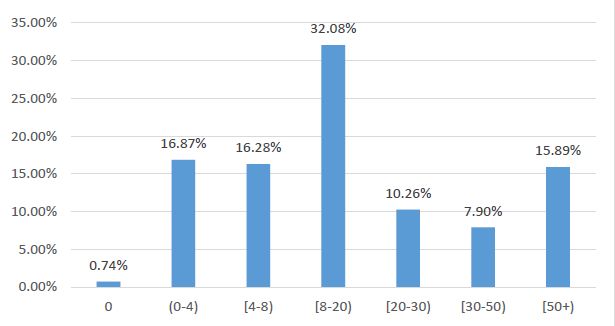
\includegraphics[width=\textwidth]{fig_22.png}
    \caption{9 P.M.}
 \label{fig_22}
\end{figure}

\subsection{One node serve ability base test}
In "Local Area Network"(LAN), different request size, different parallel request amount,
record the upload speed (KB/S)(Figure \ref{fig_28}).

\begin{figure}[htbp]
\centering
	  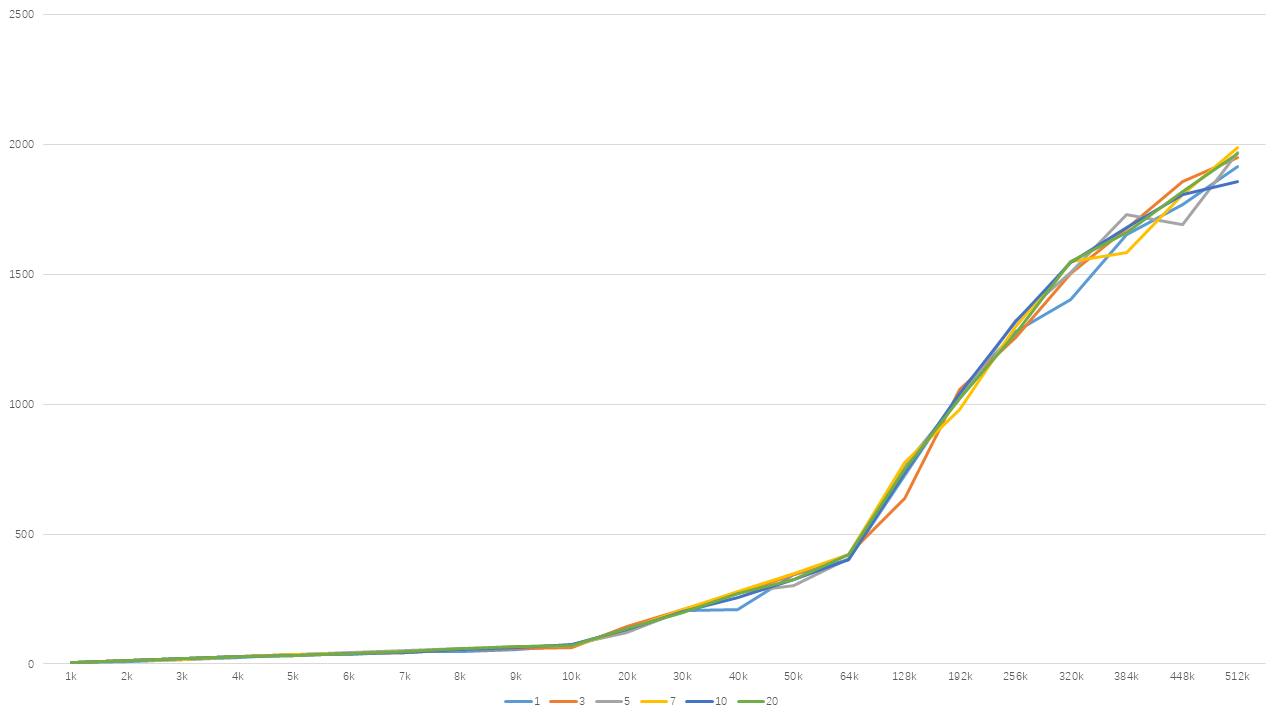
\includegraphics[width=\textwidth]{fig_28.png}
    \caption{One node serve ability base test}
 \label{fig_28}
\end{figure}

\section{File deliver test}

Random select 912 nodes, deliver file size 203M, count the downloaded nodes every 10 minutes
(Figure \ref{fig_23}).
\begin{figure}[htbp]
\centering
	  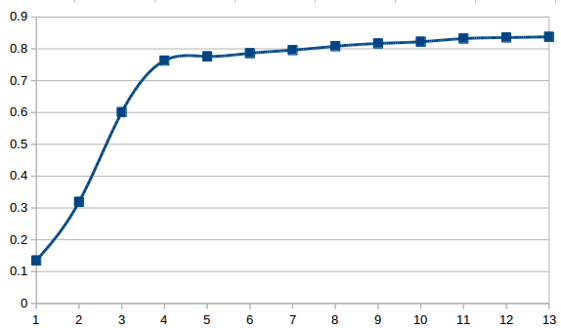
\includegraphics[width=\textwidth]{fig_23.png}
    \caption{File deliver test}
 \label{fig_23}
\end{figure}
